    
    \begin{frame}
    Mais Vu les taille des dataframes (101 colonnes juste pour MDB-Insee-divers) , il est clair que nous devions passer par une première étape consistant à reduire le nombres de variables 
    \end{frame}
    
    \begin{frame}{Resulttrain}
        
        \begin{center}
        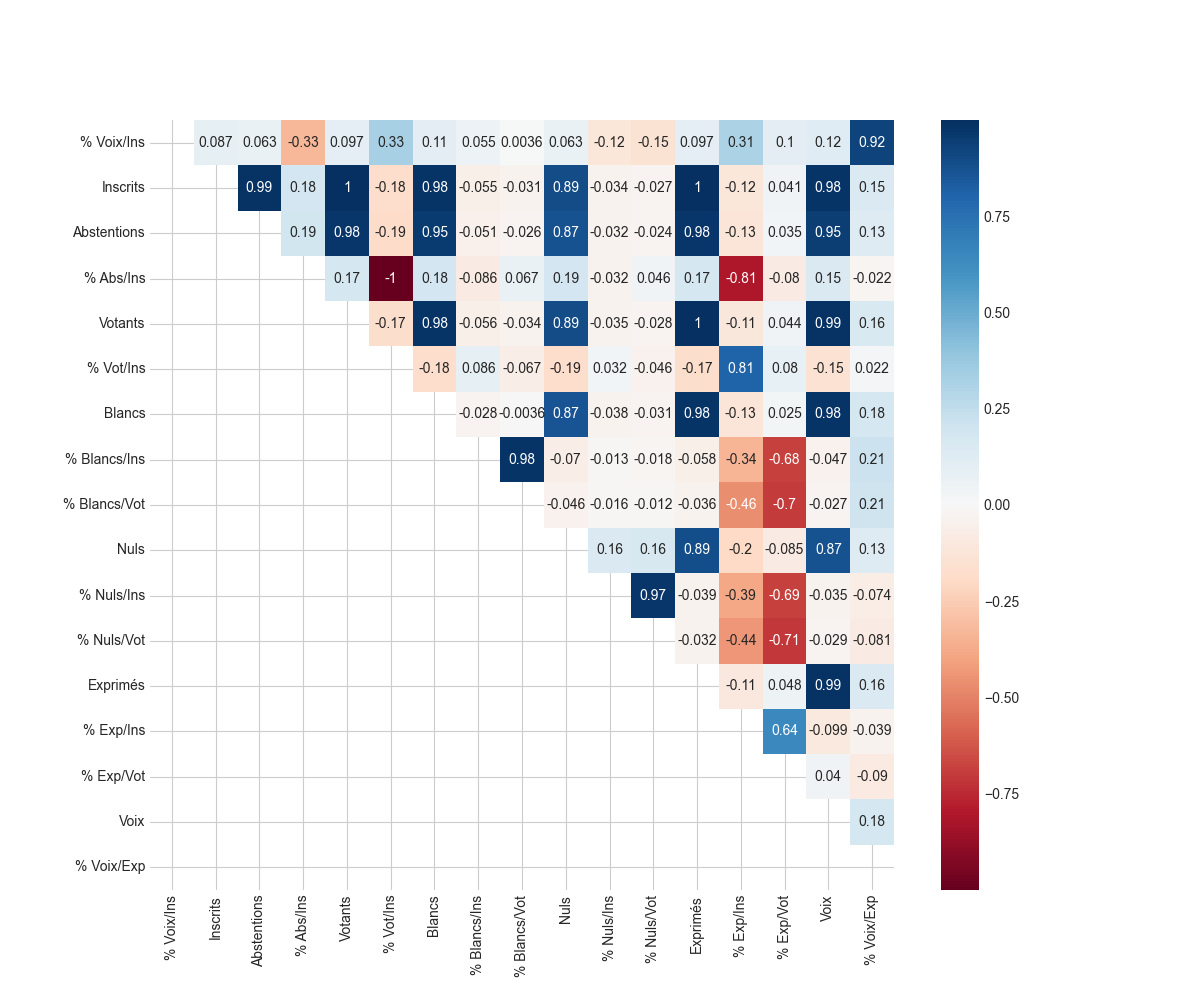
\includegraphics[width=0.8\textwidth]{figures/corr_matrix_res_train.png}
        \end{center}
        
        
    \end{frame}

    \begin{frame}{Niveau de vie}

        Aucune colonnes à supprimer 

        
        \begin{itemize}
            \item 
        \end{itemize}
    \end{frame}
